\documentclass[11pt]{article}

\newcommand{\yourname}{Kevin Zhang}

\def\comments{0}

%format and packages

%\usepackage{algorithm, algorithmic}
\usepackage{tikz}
\usepackage{algpseudocode}
\usepackage{amsmath, amssymb, amsthm}
\usepackage{tcolorbox}
\usepackage{enumerate}
\usepackage{enumitem}
\usepackage{framed}
\usepackage{verbatim}
\usepackage[margin=1.0in]{geometry}
\usepackage{microtype}
\usepackage{kpfonts}
\usepackage{palatino}
	\DeclareMathAlphabet{\mathtt}{OT1}{cmtt}{m}{n}
	\SetMathAlphabet{\mathtt}{bold}{OT1}{cmtt}{bx}{n}
	\DeclareMathAlphabet{\mathsf}{OT1}{cmss}{m}{n}
	\SetMathAlphabet{\mathsf}{bold}{OT1}{cmss}{bx}{n}
	\renewcommand*\ttdefault{cmtt}
	\renewcommand*\sfdefault{cmss}
	\renewcommand{\baselinestretch}{1.06}

\usepackage[boxruled,vlined,nofillcomment]{algorithm2e}
	\SetKwProg{Fn}{Function}{\string:}{}
	\SetKwFor{While}{While}{}{}
	\SetKwFor{For}{For}{}{}
	\SetKwIF{If}{ElseIf}{Else}{If}{:}{ElseIf}{Else}{:}
	\SetKw{Return}{Return}
	

%enclosure macros
\newcommand{\paren}[1]{\ensuremath{\left( {#1} \right)}}
\newcommand{\bracket}[1]{\ensuremath{\left\{ {#1} \right\}}}
\renewcommand{\sb}[1]{\ensuremath{\left[ {#1} \right\]}}
\newcommand{\ab}[1]{\ensuremath{\left\langle {#1} \right\rangle}}

%probability macros
\newcommand{\ex}[2]{{\ifx&#1& \mathbb{E} \else \underset{#1}{\mathbb{E}} \fi \left[#2\right]}}
\newcommand{\pr}[2]{{\ifx&#1& \mathbb{P} \else \underset{#1}{\mathbb{P}} \fi \left[#2\right]}}
\newcommand{\var}[2]{{\ifx&#1& \mathrm{Var} \else \underset{#1}{\mathrm{Var}} \fi \left[#2\right]}}

%useful CS macros
\newcommand{\poly}{\mathrm{poly}}
\newcommand{\polylog}{\mathrm{polylog}}
\newcommand{\zo}{\{0,1\}}
\newcommand{\pmo}{\{\pm1\}}
\newcommand{\getsr}{\gets_{\mbox{\tiny R}}}
\newcommand{\card}[1]{\left| #1 \right|}
\newcommand{\set}[1]{\left\{#1\right\}}
\newcommand{\negl}{\mathrm{negl}}
\newcommand{\eps}{\varepsilon}
\DeclareMathOperator*{\argmin}{arg\,min}
\DeclareMathOperator*{\argmax}{arg\,max}
\newcommand{\eqand}{\qquad \textrm{and} \qquad}
\newcommand{\ind}[1]{\mathbb{I}\{#1\}}
\newcommand{\sslash}{\ensuremath{\mathbin{/\mkern-3mu/}}}
\newcommand{\pipe}{\hspace{3pt}|\hspace{3pt}}

%mathbb
\newcommand{\N}{\mathbb{N}}
\newcommand{\R}{\mathbb{R}}
\newcommand{\Z}{\mathbb{Z}}
%mathcal
\newcommand{\cA}{\mathcal{A}}
\newcommand{\cB}{\mathcal{B}}
\newcommand{\cC}{\mathcal{C}}
\newcommand{\cD}{\mathcal{D}}
\newcommand{\cE}{\mathcal{E}}
\newcommand{\cF}{\mathcal{F}}
\newcommand{\cL}{\mathcal{L}}
\newcommand{\cM}{\mathcal{M}}
\newcommand{\cO}{\mathcal{O}}
\newcommand{\cP}{\mathcal{P}}
\newcommand{\cQ}{\mathcal{Q}}
\newcommand{\cR}{\mathcal{R}}
\newcommand{\cS}{\mathcal{S}}
\newcommand{\cU}{\mathcal{U}}
\newcommand{\cV}{\mathcal{V}}
\newcommand{\cW}{\mathcal{W}}
\newcommand{\cX}{\mathcal{X}}
\newcommand{\cY}{\mathcal{Y}}
\newcommand{\cZ}{\mathcal{Z}}

%theorem macros
\newtheorem{thm}{Theorem}
\newtheorem{lem}[thm]{Lemma}
\newtheorem{fact}[thm]{Fact}
\newtheorem{clm}[thm]{Claim}
\newtheorem{rem}[thm]{Remark}
\newtheorem{coro}[thm]{Corollary}
\newtheorem{prop}[thm]{Proposition}
\newtheorem{conj}[thm]{Conjecture}

\theoremstyle{definition}
\newtheorem{defn}[thm]{Definition}
\newtheoremstyle{case}{}{}{}{}{}{:}{ }{}
\theoremstyle{case}
\newtheorem{case}{Case}

\theoremstyle{theorem}
\newtheorem{prob}{Problem}
\newtheorem{sol}{Solution}

\tikzset{every picture/.style={line width=0.75pt}} %set default line width to 0.75pt        

\begin{document}
{\large
\noindent Name: \yourname}

\vspace{15pt}

\tikzset{every picture/.style={line width=0.75pt}} %set default line width to 0.75pt        

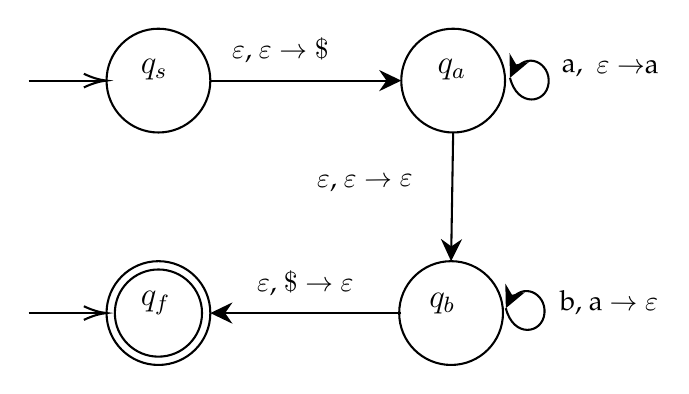
\begin{tikzpicture}[x=0.75pt,y=0.75pt,yscale=-1,xscale=1]
%uncomment if require: \path (0,199); %set diagram left start at 0, and has height of 199

%Shape: Circle [id:dp271471392298275] 
\draw   (53,44) .. controls (53,30.19) and (64.19,19) .. (78,19) .. controls (91.81,19) and (103,30.19) .. (103,44) .. controls (103,57.81) and (91.81,69) .. (78,69) .. controls (64.19,69) and (53,57.81) .. (53,44) -- cycle ;
%Shape: Circle [id:dp2021736081273684] 
\draw   (195,44) .. controls (195,30.19) and (206.19,19) .. (220,19) .. controls (233.81,19) and (245,30.19) .. (245,44) .. controls (245,57.81) and (233.81,69) .. (220,69) .. controls (206.19,69) and (195,57.81) .. (195,44) -- cycle ;
%Straight Lines [id:da9183350343495962] 
\draw    (15.5,44) -- (51,44) ;
\draw [shift={(53,44)}, rotate = 180] [color={rgb, 255:red, 0; green, 0; blue, 0 }  ][line width=0.75]    (10.93,-3.29) .. controls (6.95,-1.4) and (3.31,-0.3) .. (0,0) .. controls (3.31,0.3) and (6.95,1.4) .. (10.93,3.29)   ;
%Straight Lines [id:da5231631236234733] 
\draw    (103,44) -- (192,44) ;
\draw [shift={(195,44)}, rotate = 180] [fill={rgb, 255:red, 0; green, 0; blue, 0 }  ][line width=0.08]  [draw opacity=0] (10.72,-5.15) -- (0,0) -- (10.72,5.15) -- (7.12,0) -- cycle    ;
%Shape: Circle [id:dp9096213011848975] 
\draw   (194,156) .. controls (194,142.19) and (205.19,131) .. (219,131) .. controls (232.81,131) and (244,142.19) .. (244,156) .. controls (244,169.81) and (232.81,181) .. (219,181) .. controls (205.19,181) and (194,169.81) .. (194,156) -- cycle ;
%Curve Lines [id:da38257827769801] 
\draw    (247.38,42.66) .. controls (250.98,57.16) and (264.98,55.16) .. (265.98,45.16) .. controls (266.91,35.81) and (255.61,29.08) .. (248.74,40.1) ;
\draw [shift={(247.38,42.66)}, rotate = 294.47] [fill={rgb, 255:red, 0; green, 0; blue, 0 }  ][line width=0.08]  [draw opacity=0] (10.72,-5.15) -- (0,0) -- (10.72,5.15) -- (7.12,0) -- cycle    ;
%Straight Lines [id:da3592904350735662] 
\draw    (220,69) -- (219.05,128) ;
\draw [shift={(219,131)}, rotate = 270.92] [fill={rgb, 255:red, 0; green, 0; blue, 0 }  ][line width=0.08]  [draw opacity=0] (10.72,-5.15) -- (0,0) -- (10.72,5.15) -- (7.12,0) -- cycle    ;
%Curve Lines [id:da5279994650802105] 
\draw    (245.38,153.66) .. controls (248.98,168.16) and (262.98,166.16) .. (263.98,156.16) .. controls (264.91,146.81) and (253.61,140.08) .. (246.74,151.1) ;
\draw [shift={(245.38,153.66)}, rotate = 294.47] [fill={rgb, 255:red, 0; green, 0; blue, 0 }  ][line width=0.08]  [draw opacity=0] (10.72,-5.15) -- (0,0) -- (10.72,5.15) -- (7.12,0) -- cycle    ;
%Shape: Circle [id:dp6209857835409796] 
\draw   (53,156) .. controls (53,142.19) and (64.19,131) .. (78,131) .. controls (91.81,131) and (103,142.19) .. (103,156) .. controls (103,169.81) and (91.81,181) .. (78,181) .. controls (64.19,181) and (53,169.81) .. (53,156) -- cycle ;
%Straight Lines [id:da4734527758417679] 
\draw    (15.5,156) -- (51,156) ;
\draw [shift={(53,156)}, rotate = 180] [color={rgb, 255:red, 0; green, 0; blue, 0 }  ][line width=0.75]    (10.93,-3.29) .. controls (6.95,-1.4) and (3.31,-0.3) .. (0,0) .. controls (3.31,0.3) and (6.95,1.4) .. (10.93,3.29)   ;
%Straight Lines [id:da5459090974402354] 
\draw    (195,156) -- (106,156) ;
\draw [shift={(103,156)}, rotate = 360] [fill={rgb, 255:red, 0; green, 0; blue, 0 }  ][line width=0.08]  [draw opacity=0] (10.72,-5.15) -- (0,0) -- (10.72,5.15) -- (7.12,0) -- cycle    ;
%Shape: Circle [id:dp17662574233262274] 
\draw   (57,156) .. controls (57,144.4) and (66.4,135) .. (78,135) .. controls (89.6,135) and (99,144.4) .. (99,156) .. controls (99,167.6) and (89.6,177) .. (78,177) .. controls (66.4,177) and (57,167.6) .. (57,156) -- cycle ;

% Text Node
\draw (68,32) node [anchor=north west][inner sep=0.75pt]  [font=\large] [align=left] {$\displaystyle q_{s}$};
% Text Node
\draw (211,32) node [anchor=north west][inner sep=0.75pt]  [font=\large] [align=left] {$\displaystyle q_{a}$};
% Text Node
\draw (112,22) node [anchor=north west][inner sep=0.75pt]   [align=left] {$\displaystyle \varepsilon $, $\displaystyle \varepsilon \rightarrow \$$};
% Text Node
\draw (152.89,88.35) node [anchor=north west][inner sep=0.75pt]  [rotate=-359.31] [align=left] {$\displaystyle \varepsilon $, $\displaystyle \varepsilon \rightarrow \varepsilon $};
% Text Node
\draw (207,145) node [anchor=north west][inner sep=0.75pt]  [font=\large] [align=left] {$\displaystyle q_{b}$};
% Text Node
\draw (270.98,32.41) node [anchor=north west][inner sep=0.75pt]  [rotate=-0.45] [align=left] {a, \ $\displaystyle \varepsilon \rightarrow $a};
% Text Node
\draw (270,143.35) node [anchor=north west][inner sep=0.75pt]  [rotate=-0.58] [align=left] {b, a $\displaystyle \rightarrow \varepsilon $};
% Text Node
\draw (68,144) node [anchor=north west][inner sep=0.75pt]  [font=\large] [align=left] {$\displaystyle q_{f}$};
% Text Node
\draw (124,134) node [anchor=north west][inner sep=0.75pt]   [align=left] {$\displaystyle \varepsilon $, $\displaystyle \$\rightarrow \varepsilon $};


\end{tikzpicture}


\end{document}
